%! Author = Equipo
%! Date = 4/17/2023

% Preamble
\documentclass{beamer}
\usetheme{AnnArbor}
\usecolortheme{seahorse}
% Packages
\usepackage{amsmath}
\usepackage{adjustbox}
\usepackage{enumitem}
\usepackage{yhmath}
\usepackage{marvosym}
\usepackage{pgfplots}
\usepackage{animate}
\usepackage{cancel}
\usepackage{amssymb}
\usepackage{mathrsfs}
\usepackage[mathscr]{euscript}
\usepackage{mathtools}
\usepackage{subfig}
\usepackage{wrapfig}
\usepackage{caption}
\usepackage{sidecap}
\usepackage[spanish]{babel}
\usepackage{tcolorbox}
\usepackage[all]{xy}
\usepackage{graphicx}
\usepackage[utf8]{inputenc}
\usepackage{tabularx}
\usepackage{changepage}
\tcbuselibrary{theorems}

%Refactor commands
\renewcommand{\figurename}{Figura}
\newcommand{\invec}{\left\lbrace\begin{array}{c}}
\newcommand{\finvec}{\right\end{array}}
\newcommand{\ifff}{\Leftrightarrow}
\newcommand{\imp}{\Rightarrow}
\providecommand{\difer}[3]{\frac{\partial^{#3} #1}{\partial #2^{#3}}}
\providecommand{\abs}[1]{\left|#1\right|}
\newcommand{\commentedbox}[2]{%
  \mbox{
    \begin{tabular}[t]{@{}c@{}}
    $\boxed{\displaystyle#1}$\\
    #2
    \end{tabular}%
  }%
}
    \newcommand{\defeq}{\vcentcolon=}

%Portada
\title{Práctica 4: Medida del Campo Magnético Terrestre con Bobinas de Helmholtz}
\author{Antonio Valle Sánchez y Adolfo Enrique Vázquez}
\date{Sevilla, a 20 de abril de 2023}

% Document
\begin{document}

\maketitle
\begin{frame}{Índice}
\begin{enumerate}
    \item Introducción y objetivos
    \item Fundamento teórico
    \begin{enumerate}[label*=\arabic*.]
        \item Campo magnético creado por Bobinas de Helmholtz
        \item Medida de la componente horizontal del campo magnético terrestre
    \end{enumerate}
    \item Metodología y resultados
    \begin{enumerate}[label*=\arabic*.]
        \item Instrumentación
        \item Procedimientos y explotación de los datos
    \end{enumerate}
    \item Conclusiones y deducciones finales
    \item Cuestiones
    \item Bibliografía
\end{enumerate}
\end{frame}
\begin{frame}{1.- Objetivos}
\begin{itemize}
\item Corroborar la casi-uniformidad del campo magnético generado por una pareja de bobinas en su interior
\item Medir a raíz del factor de calibración el campo magnético terrestre en el laboratorio
\end{itemize}
\end{frame}
\begin{frame}{2.-Fundamento Teórico}
\begin{enumerate}
    \item Cálculo del campo magnético en el eje de dos bobinas coaxiales
    \item Aproximaciones de dicho valor
    \begin{enumerate}[label*=\arabic*.]
        \item Imposición de hipótesis: elección de órdenes para a y d
        \item Exactamente en el eje
        \item En un entorno del eje
        \item Relaciones entre componentes radial y axial
    \end{enumerate}
    \item Adaptación experimental: bobinado de Helmholtz
    \item Medida de la componente horizontal del campo magnético terrestre
\end{enumerate}
\end{frame}
\begin{frame}{2.1.- Cálculo del campo magnético en el eje de dos bobinas coaxiales}
    Considerando el sistema \pause \vspace{-1.5cm}\begin{figure}
        \centering
        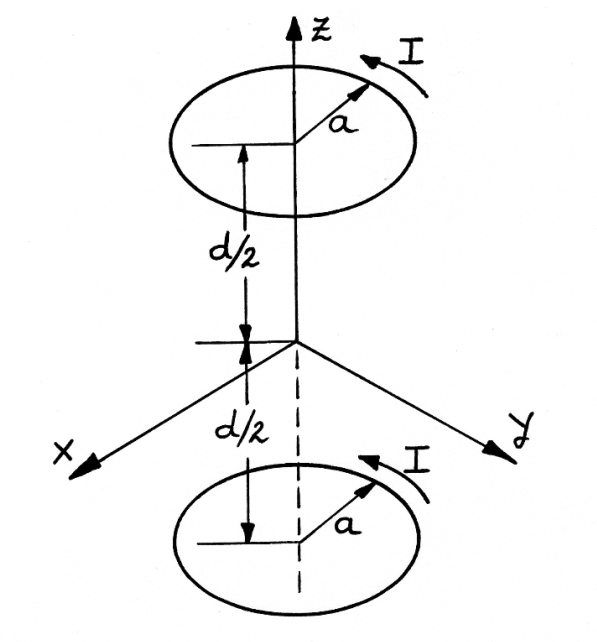
\includegraphics[scale = 0.1]{imagen_2023-04-16_100309859.png}
    \end{figure}
    Y empleando \begin{block}{Ley de Biot-Savart}
        \begin{equation}
            \vec{B}(\vec{r}) = \frac{\mu_{0}}{4 \pi} \cdot \int_{\mathcal{C}} \frac{I \cdot d\vec{l} \wedge (\vec{r} - \vec{r}')}{\abs{\vec{r} - \vec{r}'}^{3}} \nonumber
        \end{equation}
        \end{block}
\end{frame}
\begin{frame}{2.1.- Cálculo del campo magnético en el eje de dos bobinas coaxiales}
    Parametrizamos
    \begin{equation}
        \mathcal{C}_{(a,z)} \defeq \{ a \cdot \vec{u}_{\rho} + z' \cdot \vec{u}_{z} = \left( a \cdot cos(\theta') , a \cdot sin(\theta'), z' \right) \in \mathbb{R}^{3} \shortparallel \theta' \in [0,2\pi) \} \nonumber
    \end{equation}
    \pause y aplicando Ppio de Superposición sobre Biot-Savart
    \begin{align*}
        & \vec{B}(\rho = 0, z) = \frac{\mu_{0}}{4 \pi} \cdot \sum_{i \in \{-1,1\}} \left[\int_{\mathcal{C}_{\left(a,i \cdot \left( \frac{d}{2} \right) \right)}} \frac{I \cdot d\theta' \vec{u}_{\theta} \wedge (- \rho' \cdot \vec{u}_{\rho} + (z-z') \cdot \vec{u}_{z})}{\left( \rho'^{2} + (z-z')^{2} \right)^{3/2}} \right] \\
        & \ifff \commentedbox{\vec{B}(\rho = 0, z) = \frac{\mu_{0}I a^{2}}{2} \cdot \left\{ \sum_{i \in \{-1,1\}} \left[ a^{2} + \left( z + i \cdot d/2 \right)^{2} \right]^{- 3/2} \right\} \cdot \vec{u}_{z}}{}\nonumber
    \end{align*}
\end{frame}
\begin{frame}{2.2.1.- Imposición de hipótesis: elección de órdenes para a y d}
    En los casos extremos:
    \begin{itemize}
        \item $d \ll a $ : para $z \in [-d/2,d/2]$ despreciamos $(x + i \cdot d/2)^{2}$ y \pause
        \begin{itemize}
            \item 1.- $\vec{B}(\rho = 0, z) \sim \frac{\mu_{0} I }{a} \neq f(z) \imp \text{peor estimación en [-d/2,d/2]}$
            \item 2.- $\text{grandes errores relativos para mediciones de}~~z \in [-d/2,d/2]$
        \end{itemize}
\pause
        \item $d \gg a$ : para $z \in [-d/2,d/2]$ despreciamos $a^{2}$ y \pause
          \begin{itemize}
             \item 1.- $\abs{\vec{B}(\rho = 0, z)} \rightarrow \infty ~\text{para}~ z \rightarrow \pm d/2$
             \item 2.- $\text{o radios muy pequeños (mayor err rel) o dists muy grandes}$
          \end{itemize}
    \end{itemize}
\end{frame}
\begin{frame}{2.2.1.- Imposición de hipótesis: elección de órdenes para a y d}
\begin{columns}
        \column{0.4\textwidth} \begin{figure}
            \animategraphics[autoplay,loop,scale=0.25]{12}{gif1/gif1-}{0}{59}
            \caption{d crece para a fijo}
            \label{Figura 1}
        \end{figure}
        \column{0.4\textwidth} \begin{figure}
            \animategraphics[autoplay,loop,scale=0.25]{12}{gif2/gif2-}{0}{59}
            \caption{a decrece para d fijo}
            \label{Figura 2}
        \end{figure}
    \end{columns}
\end{frame}
\begin{frame}{2.2.2.- Exactamente en el eje}
    En virtud de lo anterior, es conveniente tomar $d \sim a$ y de hecho partiremos de la premisa $d = a$ \pause

    En dichas condiciones,
    \begin{equation}
        \exists~U \in \mathcal{T}_{e}(\mathbb{R}) \shortparallel 0 \in U \wedge \abs{\vec{B}(\rho = 0, z)} \in \mathcal{C}^{\infty}(U) \nonumber
    \end{equation}
    y podremos aplicar el Teorema de Taylor.\pause \\

    Teniendo en consideración que
    \begin{align*}
        & \blacksquare \vec{B}(0,0) = \frac{8\mu_{0}I}{5\sqrt{5}a} \vec{u}_{z} \nonumber \\
        & \blacksquare \frac{\partial^{j} \vec{B}}{\partial z^{j}} (0,0) = \vec{0}~\forall j \in \{1,2,3\}\\
        & \blacksquare \difer{\vec{B}}{z}{4} = - 24 \frac{144}{125a^{4}} \cdot \frac{8 \mu_{0} I}{5 \sqrt{5} a} \vec{u}_{z}\\
    \end{align*}
\end{frame}
\begin{frame}{2.2.2.- Exactamente en el eje}
    Podemos aproximar el campo en el rango $\abs{z} \in \left[ 0, \frac{a}{2} \right]$ por
    \begin{equation}
        \vec{B}(\rho=0,z) \approx \frac{8 \mu_{0} I}{5 \sqrt{5} a} \cdot \left( 1 - \frac{144}{125} \cdot \left( \frac{z}{a} \right)^{4} \right) \vec{u}_{z} \nonumber
    \end{equation}
    \pause, cuasi-constante en dicho intervalo.
\end{frame}
\begin{frame}{2.2.3.- En un entorno del eje}
    Para $\rho \ll a$ (no necesariamente nulo), empleando la relación
    \begin{equation}
        \frac{\partial B_{\rho}}{\partial \rho} (0,z) = - \frac{1}{2} \cdot \frac{\partial B_{z}}{\partial z} (0,z) \nonumber
    \end{equation}
    \pause y efectuando desarrollo de Taylor hasta orden 2, se obtiene de forma análoga
    \begin{align*}
        & B_{\rho}(\rho,z) \approx  \frac{8 \mu_{0} I}{5 \sqrt{5} a} \cdot \left(\frac{288}{125} \cdot \left( \frac{\rho}{a} \right) \cdot \left( \frac{z}{a} \right)^{3} \right)\nonumber \\
        & B_{z}(\rho,z) \approx \frac{8 \mu_{0} I}{5 \sqrt{5} a} \cdot \left( 1 - \frac{144}{125} \cdot \left( \frac{z}{a} \right)^{4} + \frac{864}{125} \cdot \left( \frac{\rho}{a} \right)^{2} \cdot \left( \frac{z}{a} \right)^{2} \right)
    \end{align*}
\end{frame}
\begin{frame}{2.2.4.- Relación entre componentes radial y axial}
    \begin{columns}
         \column{0.3\textwidth} Puesto que\begin{itemize}
        \item $\rho \ll a$
        \item $\abs{z} \leq \frac{a}{2}$
        \end{itemize} \pause
         \column{0.1\textwidth} $\Longrightarrow$
         \column{0.5\textwidth} \begin{itemize}
        \item $\frac{288}{125} \cdot \left( \frac{\rho}{a} \right) \cdot \left( \frac{z}{a} \right)^{3} \ll 1 $
        \item $1 \gg \frac{144}{125} \cdot \left( \frac{z}{a} \right)^{4}, \frac{864}{125} \cdot \left( \frac{\rho}{a} \right)^{2} \cdot \left( \frac{z}{a} \right)^{2} $
        \end{itemize}
    \end{columns}
    \pause
    inferimos que $\exists \varepsilon > 0 \shortparallel$
    \begin{equation}
         \commentedbox{\vec{B}(\rho,z) = \frac{8 \mu_{0} I}{5 \sqrt{5} a} \vec{u}_{z}}{}\nonumber
    \end{equation}
    es una estimación asumible en el recinto  \vspace{-1.5cm}\begin{figure}
        \hspace{8cm}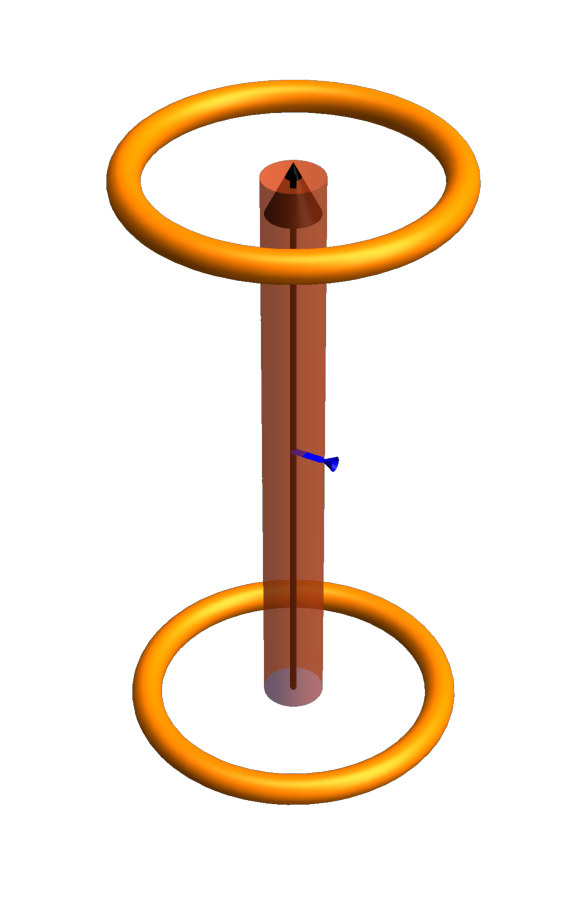
\includegraphics[scale=0.3]{CYLELMOP4V2.pdf}
    \end{figure}
\end{frame}
\begin{frame}{2.3.- Adaptación experimental: bobinado de Helmholtz}
    Para I moderadas, $\abs{\vec{B}} \ll 1 T$ en el recinto dado.

    Se opta por el bobinado de ambas espiras (\emph{Bobinas de Helmholtz}):

    \begin{equation}
        \vec{B}_{H} \approx N \cdot \frac{8 \mu_{0} I}{5 \sqrt{5} \overline{a}}\nonumber
    \end{equation}
\end{frame}
\begin{frame}{2.4.- Medida de la componente horizontal del campo magnético terrestre}
    \begin{figure}
        \centering
        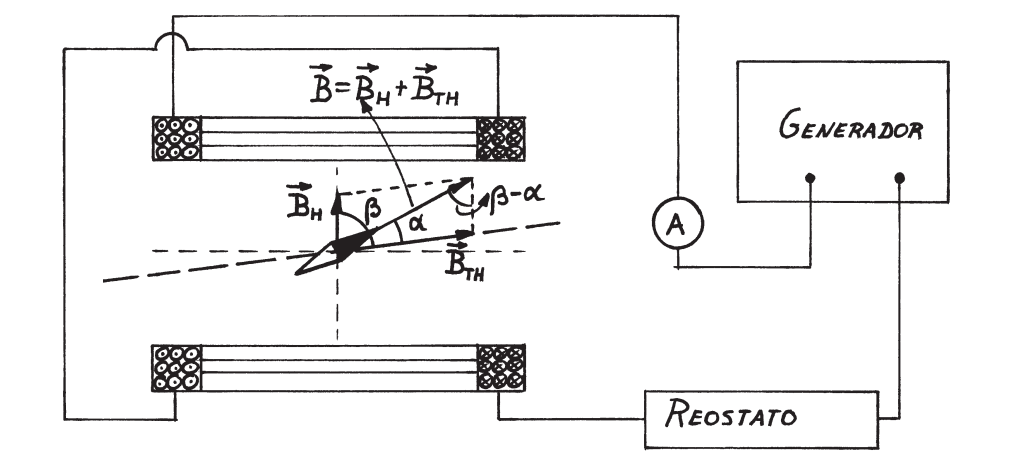
\includegraphics[scale=0.35]{imagen_2023-04-17_035041851.png}
        \label{fig:my_label}
    \end{figure}
\cite{Boix}
\end{frame}
\begin{frame}{2.4.- Medida de la componente horizontal del campo magnético terrestre}
En virtud del Teorema del seno, \pause
    \begin{align*}
        & \frac{\abs{B_{H}}}{sin(\alpha)} = \frac{\abs{B_{TH}}}{sin(\beta-\alpha)} \nonumber \ifff
        & \abs{I_{H}} = \frac{\abs{B_{TH}}}{K_{H}} \cdot \frac{sin(\alpha)}{sin(\beta - \alpha)}
    \end{align*}
\end{frame}
\begin{frame}{3.- Metodología y Resultados}
\begin{enumerate}
\item Instrumentación
\item Procedimientos y explotación de los datos
\begin{enumerate}[label*=\arabic*.]
    \item Cuasi-constancia del campo a lo largo de los ejes Z e Y
    \item Calibrado
    \item Componente horizontal
    \item Componente vertical
    \end{enumerate}
\end{enumerate}
\end{frame}
\begin{frame}{3.1.- Intrumentación}
 \begin{figure}
  \includegraphics[scale=0.4]{Instrumentación.JPG}
  \end{figure}
\cite{UGR}
\end{frame}
\begin{frame}{3.2.1- Cuasi-constancia del campo a lo largo de los ejes Z e Y}
 \begin{figure}
  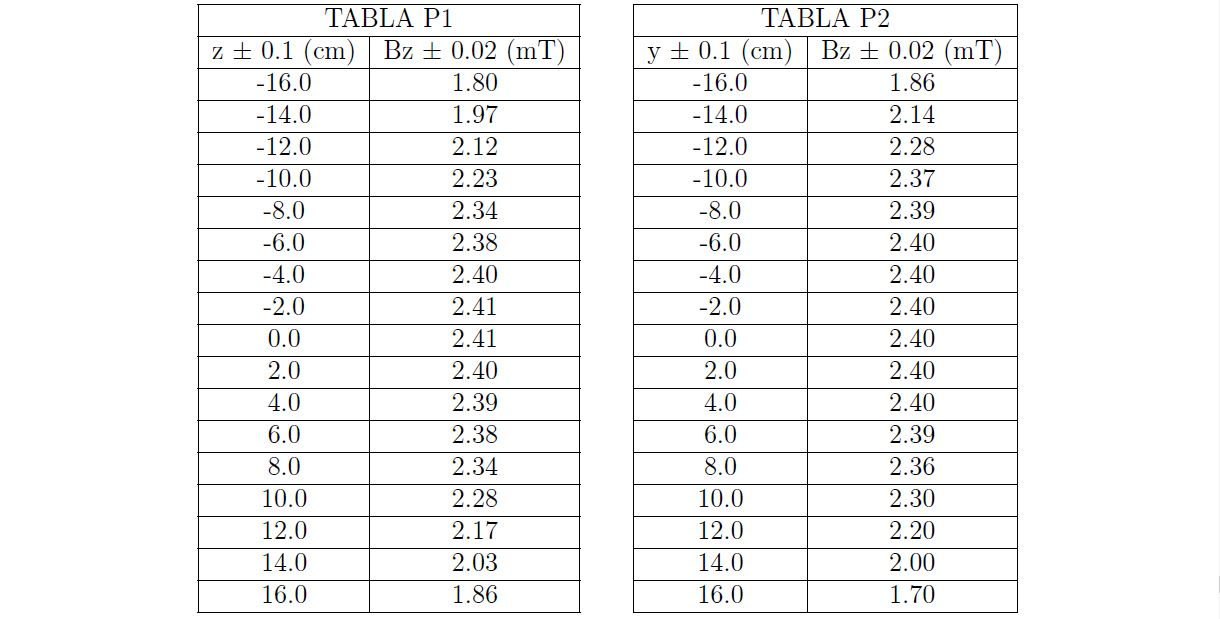
\includegraphics[scale=0.4]{TablaPuta.JPG}
  \end{figure}
\end{frame}
\begin{frame}{3.2.1- Cuasi-constancia del campo a lo largo de los ejes Z e Y}
    \begin{columns}
        \column{0.45\textwidth} \begin{figure}
            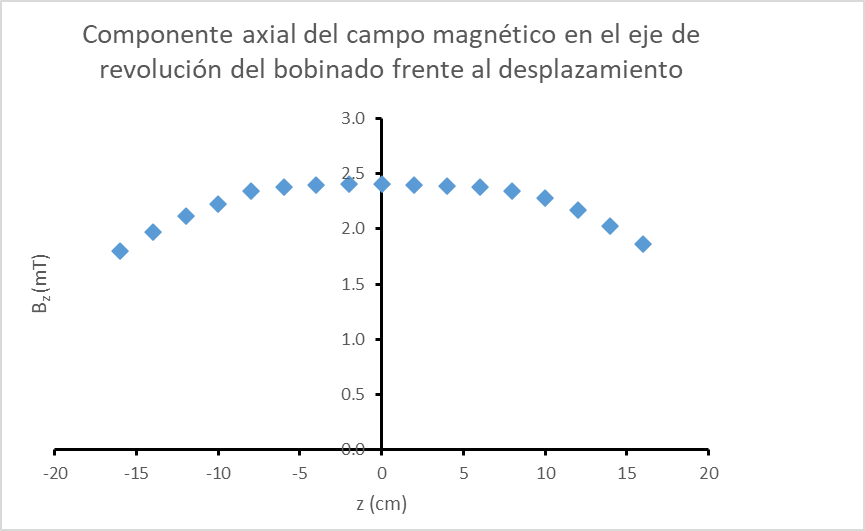
\includegraphics[scale=0.4]{image0.png}
            \label{fig:my_label}
        \end{figure}
        \column{0.45\textwidth} \begin{figure}
            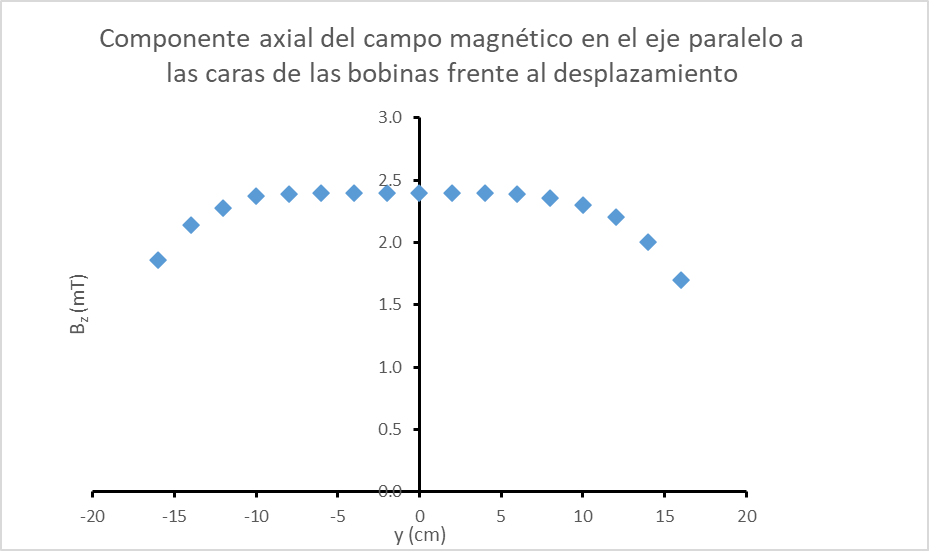
\includegraphics[scale=0.4]{image1.png}
            \label{fig:my_label}
        \end{figure}
    \end{columns}
\end{frame}
\begin{frame}{3.2.2.- Calibrado}
    \begin{table}[]
\begin{tabular}{|c|c|}
\hline
I ± 0.1 (A) & Bh ± 0.01 (mT) \\ \hline
0.2         & 0.09           \\ \hline
0.4         & 0.24           \\ \hline
0.6         & 0.38           \\ \hline
0.8         & 0.51           \\ \hline
1.0         & 0.65           \\ \hline
1.2         & 0.80           \\ \hline
1.4         & 0.93           \\ \hline
1.6         & 1.08           \\ \hline
1.8         & 1.21           \\ \hline
2.0         & 1.35           \\ \hline
\end{tabular}
\end{table}
\end{frame}
\begin{frame}{3.2.2.- Calibrado}
    \begin{figure}
        \centering
        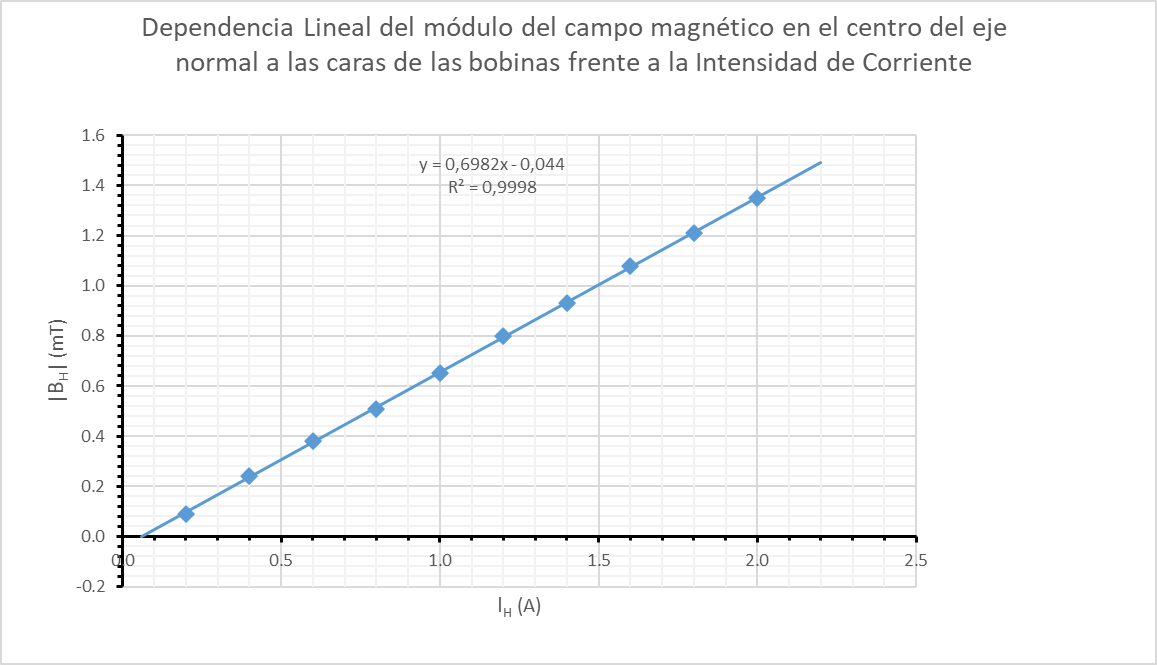
\includegraphics[scale=0.6]{image2.png}
        \label{fig:my_label}
    \end{figure}
\end{frame}
\begin{frame}{3.2.2.- Calibrado}
    , de donde se sigue
    \begin{equation}
        \commentedbox{K_{H} \pm \Delta K_{H}}{} \equiv \text{pendiente} \pm \Delta \text{pendiente} = \commentedbox{0.698 \pm 0.003 mT \cdot A^{-1}}{} \nonumber
    \end{equation}
\end{frame}
\begin{frame}{3.2.3.- Componente horizontal}
    Escogiendo $\beta = \pi/2$, se tiene $sin(\alpha - \beta) = cos(\alpha)$ y \pause
    \begin{equation}
        \abs{I_{H}} = \frac{\abs{B_{H}}}{K_{H}} \cdot tan(\alpha)\nonumber
    \end{equation}
\end{frame}
\begin{frame}{3.2.3.- Componente horizontal}
    \begin{table}[]
\begin{tabular}{|c|c|c|}
\hline
$\alpha \pm 1$ (degs) & $tan(\alpha)$      & $I_{H} \pm 0.1$ (mA) \\ \hline
20        & 0.363970234 & 8.3     \\ \hline
25        & 0.466307658 & 11.2    \\ \hline
30        & 0.577350269 & 13.7    \\ \hline
35        & 0.700207538 & 16.8    \\ \hline
40        & 0.839099631 & 20.1    \\ \hline
45        & 1           & 24      \\ \hline
50        & 1.191753593 & 28.5    \\ \hline
55        & 1.428148007 & 33.7    \\ \hline
60        & 1.732050808 & 41      \\ \hline
65        & 2.144506921 & 50      \\ \hline
70        & 2.747477419 & 66.8    \\ \hline
\end{tabular}
\end{table}
\end{frame}
\begin{frame}{3.2.3.- Componente horizontal}
    \begin{figure}
        \centering
        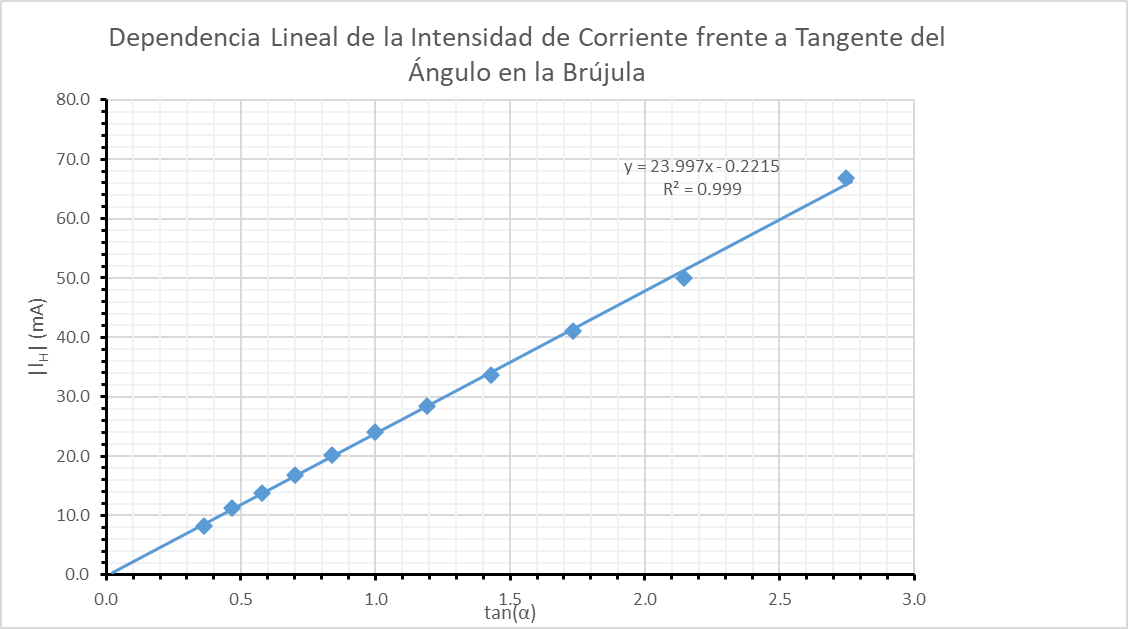
\includegraphics[scale=0.5]{image3.png}
        \label{fig:my_label}
    \end{figure}
\end{frame}
\begin{frame}{3.2.3.- Componente horizontal}
    Puesto que se conoce $K_{H} \pm \Delta K_{H}$ y \pause
    \begin{align*}
        &\abs{B_{H}} \pm Delta \abs{B_{H}} = K_{H} \cdot \text{pendiente} + (\text{pendiente} \cdot \Delta K_{H} + K_{H} \cdot \Delta \text{pendiente}) \nonumber \\
        &\iff \commentedbox{\abs{B_{H}} + \Delta \abs{B_{H}} = 16.75 \pm 0.25 \mu T }{}
    \end{align*}
\end{frame}
\begin{frame}{3.2.4.- Componente vertical}
Finalmente, se han medido dos ángulos que forma el campo con la horizontal
\begin{itemize}
\item $\gamma_{1} = 74 \pm 1$ (degs)
\item $\gamma_{2} = 58 \pm 1$ (degs)
\end{itemize}
\pause Tomando media, $\overline{\gamma} = 66 \pm 2 (degs)$. \pause

Puesto que $tan(\overline{\gamma}) = \frac{\abs{B_{TV}}}{\abs{B_{TH}}}$, se tiene \pause

\begin{align*}
& \abs{B_{TV}} \pm \Delta \abs{B_{TV}} = \\
& = (\abs{B_{TH}} \cdot \tan(\overline{\gamma})) \pm \left( \Delta \abs{B_{TH}} \cdot tan(\overline{\gamma}) + \abs{B_{TH}} \cdot sec^{2}(\overline{\gamma}) \cdot \Delta \overline{\gamma} \right) \\
& \iff \commentedbox{\abs{B_{TV}} \pm \Delta \abs{B_{TV}} = 38 \pm 4 \mu T}{}
\end{align*}
\end{frame}
\begin{frame}{4.- Conclusiones}
\begin{itemize}
\item En efecto, en el interior de los solenoides el campo es casi uniforme en una región extensa
\item Comparación con datos de NOAA \cite{NOAA}:
\begin{align*}
 & \abs{B_{TH,NOAA}} = 27,40 \pm 0,13 \mu T \\
 & \abs{B_{TV,NOAA}} = 33,90 \pm 0,16 \mu T \nonumber
\end{align*}
\end{itemize}
\end{frame}
\begin{frame}{5.- Cuestiones}
\begin{figure}
        \centering
        \includegraphics[width = \textwidth, height = 0.7\textheight]{Cuestiones.JPG}
    \end{figure}
\end{frame}
\begin{frame}{Referencias}
\bibliographystyle{IEEEtran}
\bibliography{refs}
\end{frame}
\end{document}

